\section{Fase di boot}
La prima fase dell'esecuzione di un sistema P2P distribuito è quella di boot, ossia di inizializzazione del sistema. I peer che vogliono entrare nella rete comunicano con il server di bootstrap, il quale fornirà loro una lista parziale di IP dei superpeer a cui connettersi.\linebreak
Allo stesso modo i superpeer avranno una loro fase di boot, nella quale, comunicheranno al server di bootstrap il loro ingresso nella rete.\linebreak 

\subsection{Peer}

\subsubsection{Join al server di bootstrap}
Il peer per connettersi alla rete deve contattare il server di boostrap. Questa operazione (detta di \textit{join}) è fondamentale per il corretto funzionamento del peer, il quale deve essere sicuro di ricevere le informazioni per poter essere eseguito correttamente.
La \textit{join} al server è molto semplice, viene instaurata una connessione TCP tra le due entità, le cui scambieranno dei messaggi.\linebreak
\begin{figure}[h]
\centering
\subfigure[Lista non vuota]
{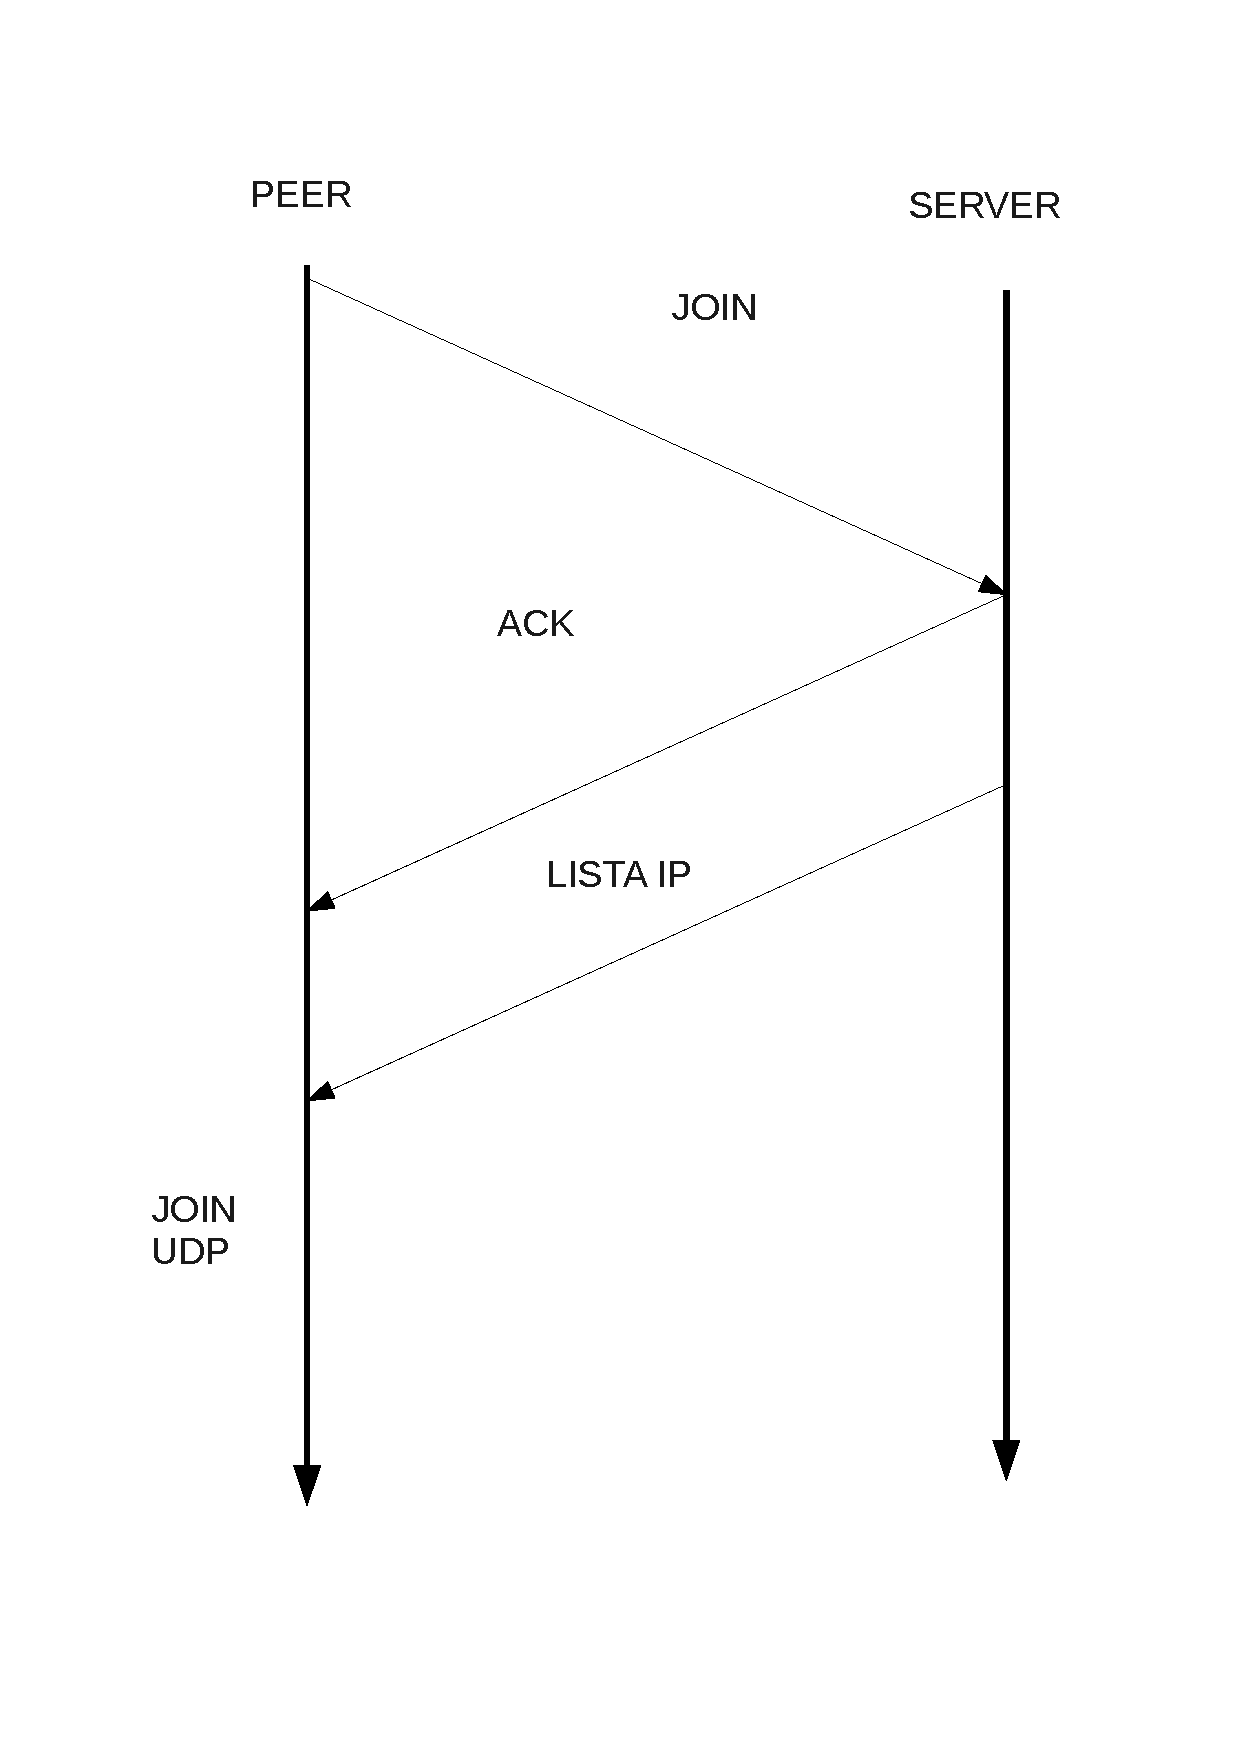
\includegraphics[width=5cm]{img/join1}}
\subfigure[Lista vuota]
{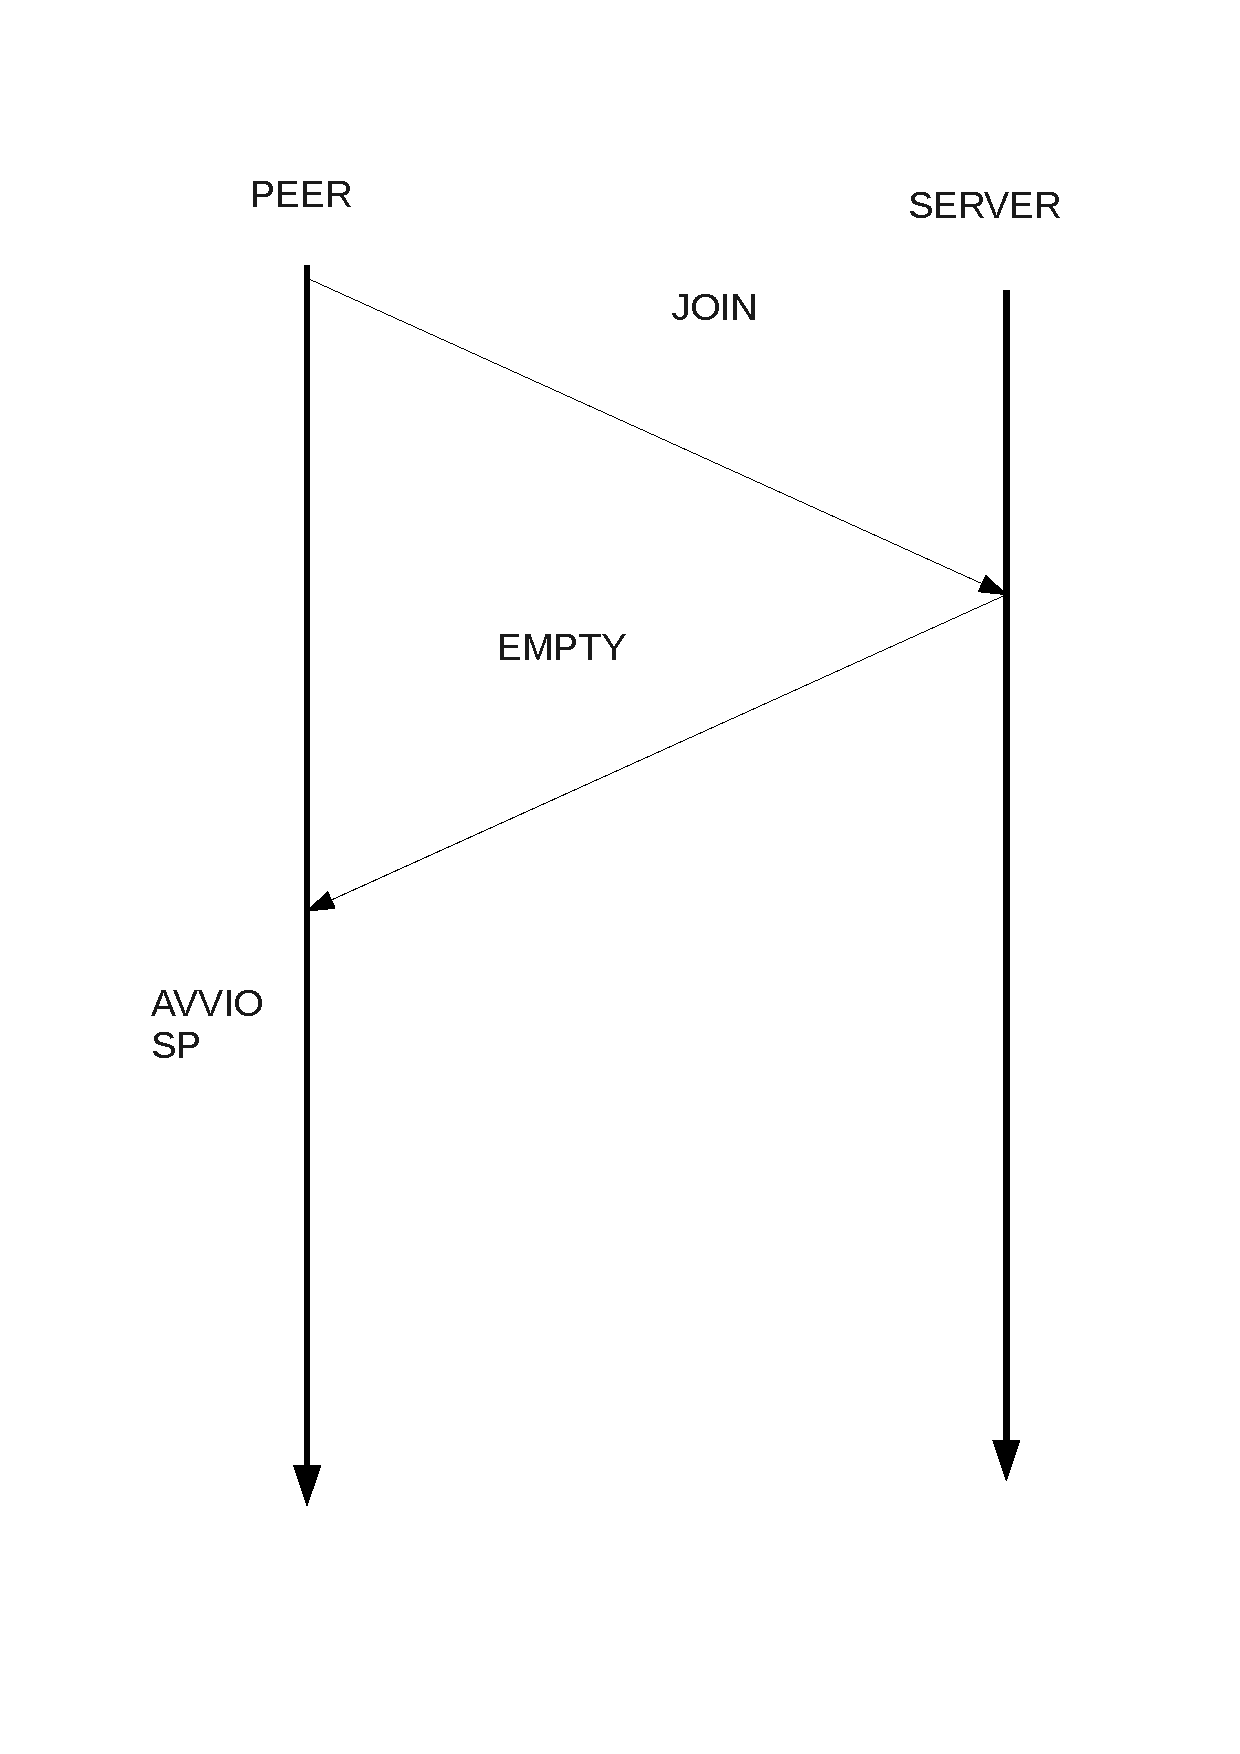
\includegraphics[width=5cm]{img/join2}}
\caption{Join del peer al server di bootstrap\label{join}}
\end{figure}
\linebreak
Come si può vedere in figura \ref{join}, il peer, dopo essersi connesso, invierà un messaggio di "join", il quale verrà letto e processato dal server. Quest'ultimo scandirà la lista dei superpeer presenti nella rete e risponderà al peer, fornendogli i riferimenti ad essi. Informerà inoltre il peer del fatto che esso debba diventare un superpeer o no.\linebreak
Sono quindi possibili due scenari:
\begin{itemize}
\item La lista dei superpeer è vuota
\item La lista contiene almeno un superpeer
\end{itemize}
Nel primo caso il peer che effettua la join verrà eletto automaticamente superpeer dal server, il quale manderà al peer un messaggio di "empty" per comunicare che la lista è vuota. Il peer che è stato eletto superpeer dovrà effettuare una seconda fase di boot riguardante l'inizializzione del superpeer.\linebreak
Nel secondo caso invece, il peer riceverà un messaggio di "ack", seguito da una lista di IP ai quali può connettersi. Inizierà a questo punto la fase di join al superpeer.\linebreak
I messaggi scambiati in questo caso non sono strutturati, ma sono semplici stringhe inviate nella rete ("join", "ack", "empty"). Al contrario, gli ip inviati dal server al peer sono degli interi long che identificano l'ip del superpeer nel formato di rete.\linebreak

\subsubsection{Join udp al superpeer}
Il peer che vuole connettersi ad uno dei superpeer presenti nella lista ricevuta dal server, cercherà di compiere la scelta localmente migliore, contattando il superpeer geograficamente più vicino tra quelli disponibili. \linebreak
Per potersi “connettere” al superpeer migliore, il peer effettuerà quindi un ping (utilizzando \textit{ping\_UDP}) su tutti gli ip restituiti e li ordinerà in base al miglior tempo di risposta. Dopo aver deciso un ordine di preferenza tra i vari superpeer, proverà a connettersi al miglior superpeer possibile tramite un operazione di \textit{join\_UDP}.  \linebreak
Tale operazione è molto importante in quanto permette di creare una "connessione" logica con il superpeer, il quale riceverà dal peer le informazioni sui file condivisi contenute in un filtro di bloom. \linebreak
Le operazioni di ping\_UDP e join\_UDP, essendo basate sul protocollo UDP, presentano vantaggi e svantaggi che le operazioni su TCP non hanno. 
\linebreak\linebreak
	\begin{figure}[h]
	\centering
	\subfigure[Ping del peer ai superpeer e successiva join\_UDP al superpeer scelto \label{sel_sp}]
	{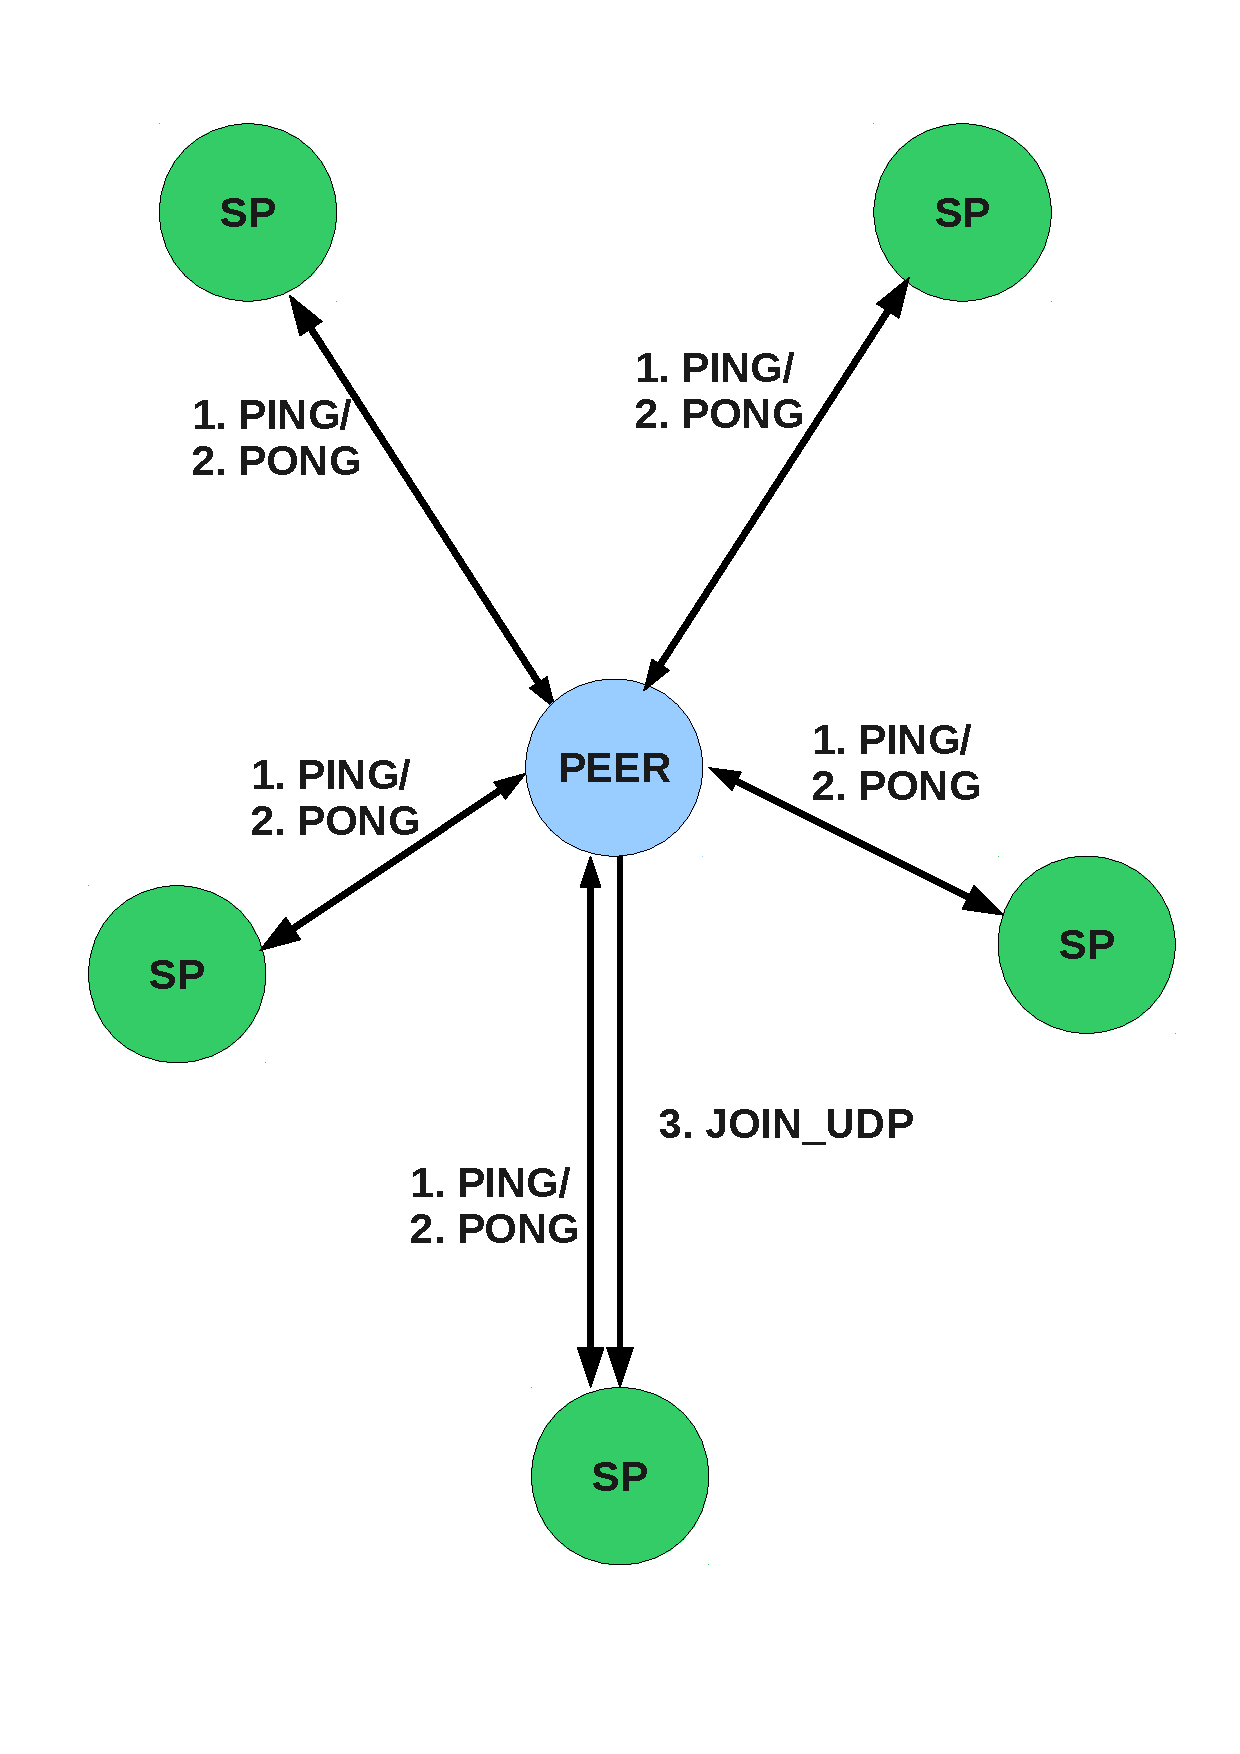
\includegraphics[width=6cm]{img/peer-sp}}
	\subfigure[Ping del peer al superpeer\label{ping_udp}]
	{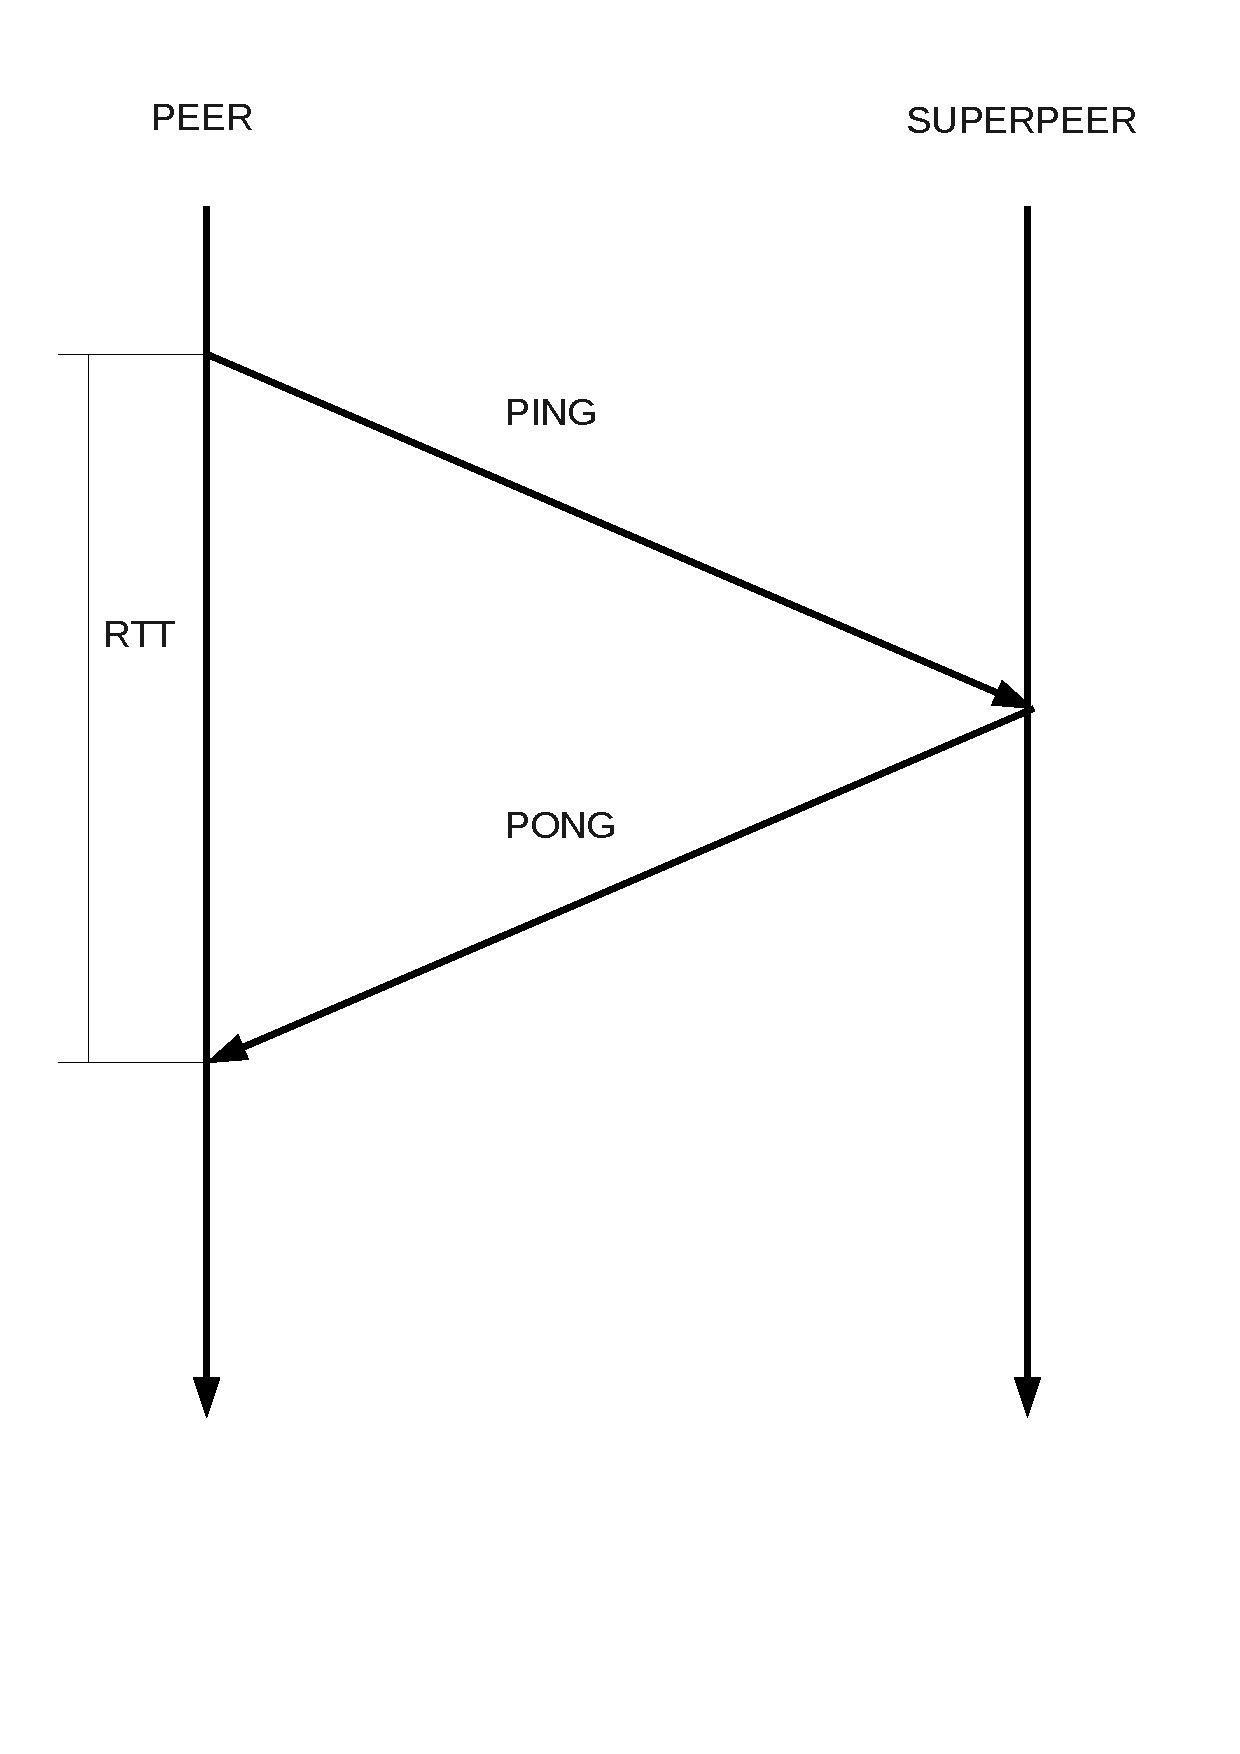
\includegraphics[width=6cm]{img/ping_udp}}
	\caption{Fase di boot del peer\label{bootpeer}}
\end{figure}


\textbf{PING\_UDP}\linebreak
L'operazione di ping\_UDP è molto utile, in quanto viene usata per misurare il tempo di risposta di un superpeer (come nel caso della fase di boot di un peer) o per refreshare le informazioni di un peer o un superpeer.\linebreak
Nel chiamare la funzione ping\_UDP, il peer specifica su quale IP effettuare il ping. Questo comando viene inviato al superpeer tramite un unico segmento udp strutturato in un pacchetto come indicato precedentemente nei dettagli architetturali del peer.\linebreak
In questa operazione il campo command è ovviamente impostato a "ping", mentre l'unico dato aggiuntivo del pacchetto è il rating del peer che invia il ping. Il rating viene inviato insieme al ping in modo tale da aggiornare le informazioni che il superpeer possiede del peer.\linebreak
Tale aggiunta al messaggio di ping è dovuta dal fatto che il superpeer così non ha solo l'informazione sui file contenuti nei peer, ma ha anche una panoramica della loro qualità. Queste informazioni possedute dal superpeer sono molto utili per la gestione dinamica della rete, ma per questo aspetto si rimanda allo specifico capitolo.\linebreak
\linebreak
\textbf{JOIN\_UDP} \linebreak
L'operazione di join\_UDP permette al peer di instaurare una "connessione" logica con il superpeer. Il peer, che chiamerà questa funzione, invierà al superpeer un messaggio UDP strutturato di join. Tale messaggio è strutturato, come tutti gli altri messaggi UDP che vengono scambiati tra peer e superpeer, da tre campi: comand, size e dati. Nella join\_UDP il campo comand è impostato a "join" (da non confondere con il messaggio NON strutturato tcp di join), e nel campo dati viene salvato il filtro di bloom del peer e il suo rating.\linebreak
Il superpeer che riceve un messaggio di join\_UDP deve innanzi tutto controllare la sua disponibilità ad accettare connessioni, quindi se il numero di peer connessi ad esso non avranno raggiunto il valore massimo di riferimento NUMERO\_MAX\_PEER allora il superpeer accetterà il nuovo peer. Ovviamente se il peer è già connesso al superpeer la join verrà usata unicamente per aggiornare le informazioni di tale peer (ad esempio il comando update, che non fà altro che chiamare la join\_UDP).


\begin{figure}[h]
	\centering
	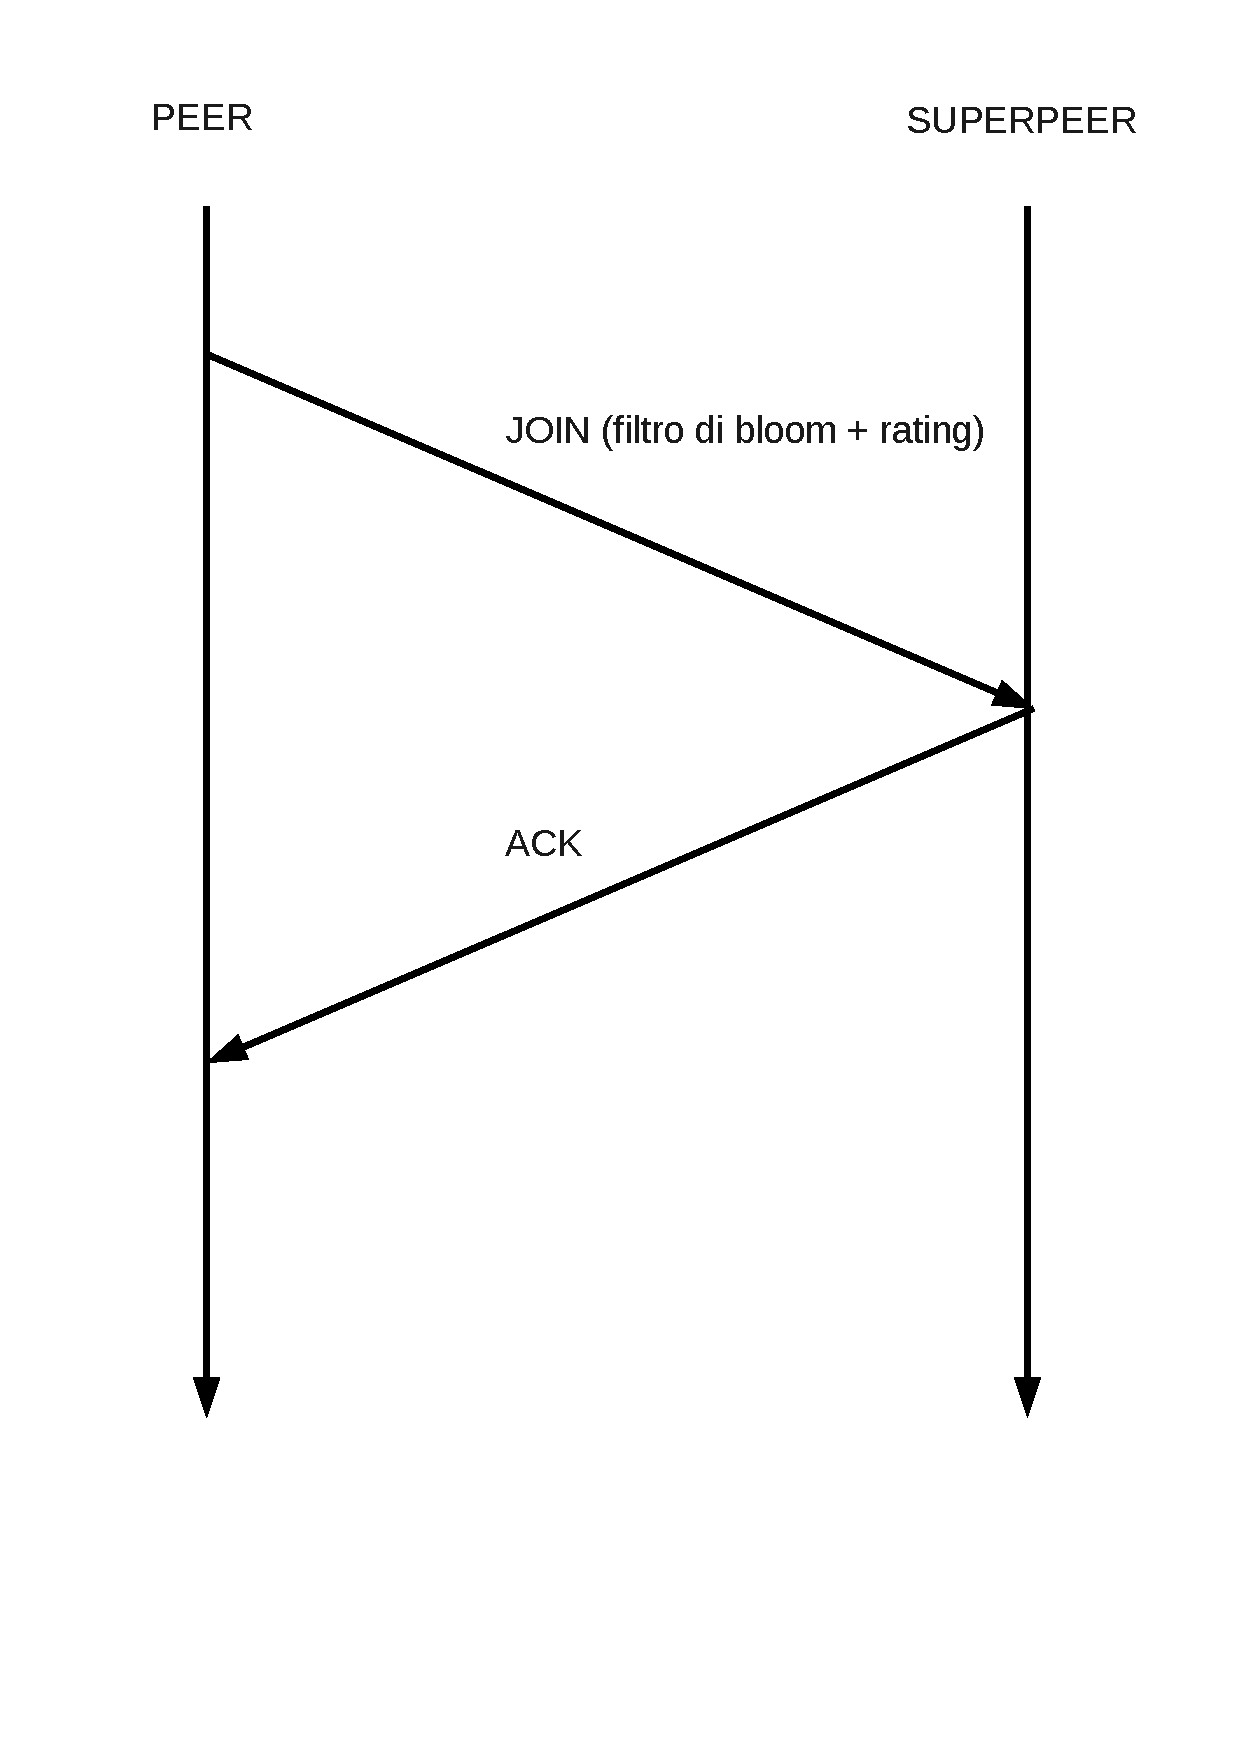
\includegraphics[width=5cm]{img/join_udp}
	\caption{Join del peer al superpeer\label{join_udp}}
\end{figure}

\begin{figure}[h]
	\centering
	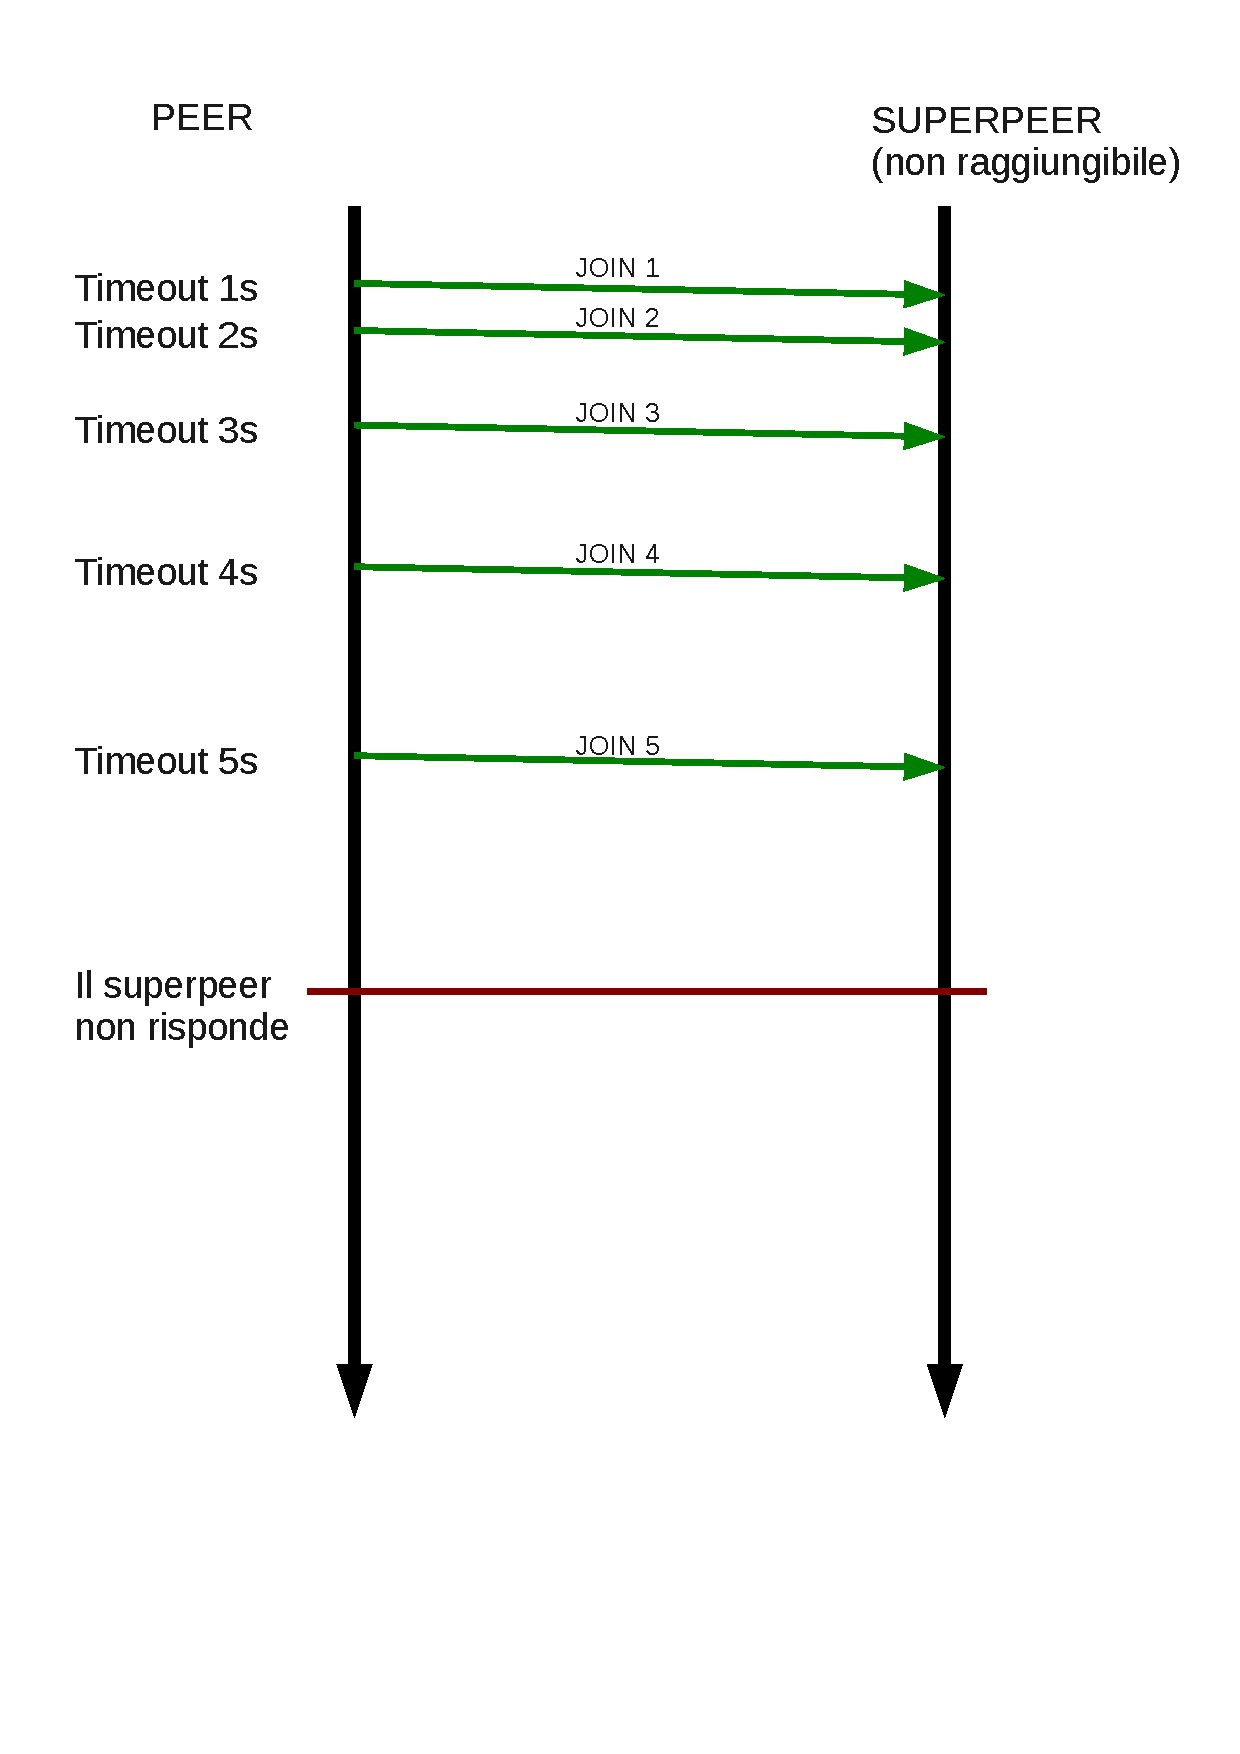
\includegraphics[width=7cm]{img/join_timeout}
	\caption{Join del peer a un superpeer non raggiungibile, gestione timeout\label{join_timeout}}
\end{figure}

Poichè la comunicazione su cui si basa lo scambio di messaggi tra peer e superpeer è di tipo UDP, i messaggi saranno di numero limitato e quindi non appesantiranno la rete. Il problema dell'UDP però è che non si hanno sicurezze sull'arrivo dei messaggi, quindi non si può avere neanche la sicurezza riguardo all'esecuzione di un superpeer.\linebreak
Il peer che chiama la join\_UDP utilizza un semplice sistema di timer interno all'operazione così da evitare che il peer rimanga in attesa per un tempo troppo lungo di una risposta da un superpeer, il quale potrebbe anche non rispondere mai.\linebreak
Dopo aver mandato il messaggio strutturato, il peer avvierà un timer (utilizzando il segnale di SIGALRM inviato dalla chiamata di sistema alarm(t) dopo un tempo t): se entro un certo tempo non arriverà alcuna risposta, la join\_UDP proverà a rifare la join per cinque volte. Nello scenario in cui non esista il superpeer che si vuole contattare, il peer proverà a contattare per cinque volte il superpeer scelto; tuttavia nei diversi tentativi di contattare il superpeer il timeout non sarà costante, bensì aumenterà ad ogni nuova chiamata della funzione, in modo tale da non occupare la rete con tanti messaggi ravvicinati e per far sì che, anche se la rete è congestionata ma il superpeer è in realtà connesso, quest'ultimo abbia il tempo di rispondere (vedere figura \ref{join_timeout}).\linebreak

\subsection{Superpeer}
\subsubsection{Register del superpeer al server di bootstrap}
Il peer che viene eletto superpeer dovrà effettuare per prima cosa un operazione detta di \textit{register}, la quale consiste nell'informare il server della sua presenza nella rete e nella disponibilità ad interagire con i peer che si connetteranno successivamente.\linebreak
Questa operazione, al pari della join del peer al server, è molto semplice: il superpeer invia un messaggio di "register" al quale il server risponderà con "empty" nel caso non ci siano superpeer connessi, o con "ack" seguito da una lista di ip di altri superpeer.\linebreak
Il server che riceve una register, oltre a rispondere con "ack" o "empty" (come nel caso della join del peer), inserirà nella sua lista di superpeer l'ip di quello che sta effettuando la register.\linebreak
\linebreak
Un altra differenza rispetto alla join del peer è che la lista di ip restituita viene usata dal superpeer per creare una rete di overlay con altri superpeer, con i quali poter comunicare per gestire la rete ed effettuare ricerche.\linebreak
Nonostante lo scambio di messaggi tra superpeer e server è totalmente analogo alla join del peer, le due operazioni vengono usate per scopi molto diversi: la join serve al peer solo per poter trovare un superpeer al quale collegarsi, la register invece serve per inizializzare il superpeer il quale, con le informazioni ricevute dal server, creerà la rete sulla quale avverranno tutte le operazioni.\linebreak

\subsubsection{Entrata del superpeer nella rete d'overlay}
Dopo aver effettuato la register al server di bootstrap il superpeer inizia a provare ad aprire al più 3(il numero massimo di vicini è stato impostato a 6) connessioni TCP con gli indirizzi dei superpeer attivi ottenuti dal bootstrap i quali possono accettare la connessione rispondendo con un ack e instaurando di fatto la connessione TCP permanente presente tra vicini.\linebreak
In caso il superpeer che riceve la join ha esaurito le connessioni TCP disponibili(è già connesso a 6 superpeer), risponderà al messaggio di join con un messaggio di "full" il quale inoltre conterrà gli indirizzi IP dei propri vicini che non hanno esaurito le connessioni (se presenti), dopo di chè chiuderà la connessione TCP, il superpeer che riceve in risposta un messaggio di "full" proverà a contattare i superpeer ricevuti in risposta insieme al messaggio di full (se presenti) inoltrando a loro la join, questo finchè non riesce ad instaurare almeno 3 connessioni TCP oppure non ci sono più superpeer a cui effettuare la join.\linebreak
La scelta di instaurare al più 3 connessioni TCP e non direttamente tutte e 6 all'inizio è stata fatta per evitare una situazione di stallo in cui tutti i superpeer hanno tutti il numero massimo di connessioni TCP già attive e di conseguenza un nuovo superpeer che arriva rimarrebbe al di fuori della rete di overlay e mano a mano che arrivano nuovi superpeer (se non si dovessero scollegare superpeer) 
si verrebbe a creare una rete di overlay completamente indipendente da quella che ha tutte le connessioni TCP già attive, e questo potenzialmente si potrebbe verificare più volte, causando la creazione di più reti overlay separate.\linebreak


